In order to assess the influence of interface conditions on the outgassing flux, simulations are performed with chemical potential continuity (Equation \ref{eq: c/s conservation}) or mobile concentration continuity assuming in both cases flux conservation (Equation \ref{eq: flux conservation}).
For the sake of simplicity and to emphasis on the influence of interface conditions, no trapping was assumed and idea Dirichlet boundary conditions were set.
Simulations were performed on two test cases: W/Cu and Cu/EUROFER.
The materials properties used for the simulations can be found in Table \ref{tab:materials properties_1}.
In both cases the solute concentration $c_\mathrm{m}$ was set to \SI{1e20}{m^{-3}} at $x=0$ and zero on the other boundary.

\subsection{W/Cu case}
A \SI{4}{mm}-thick slab made of \SI{2}{mm} of W (referred as $\Omega_1$) and \SI{2}{mm} of Cu (referred as $\Omega_2$)  at $T=\SI{500}{K}$ was first simulated.



\begin{figure*}
    \centering
    \subfloat[Solute profiles at steady state (W/Cu)]{%
        \label{fig: solute profiles w cu}
        \begin{overpic}[width=0.5\linewidth]{Figures/Chapter3/monoblocks/interface_condition/w_cu/solute_profiles.pdf}
            \put(35, 55){W}
            \put(65, 35){Cu}
        \end{overpic}
    }
    \subfloat[Outgassing flux (W/Cu)]{%
        \label{fig: outgassing flux w cu}
        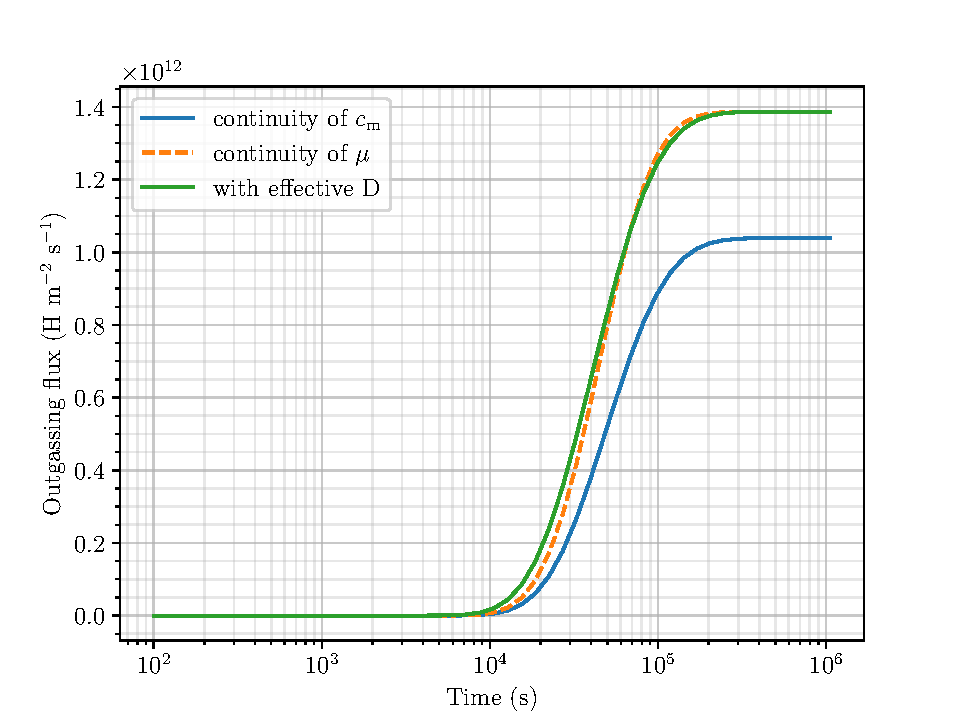
\includegraphics[width=0.5\linewidth]{Figures/Chapter3/monoblocks/interface_condition/w_cu/comparison_fluxes.pdf}
    } \\
    \subfloat[Solute profiles at steady state (Cu/EUROFER)]{%
        \label{fig: solute profiles cu eurofer}
        \begin{overpic}[width=0.5\linewidth]{Figures/Chapter3/monoblocks/interface_condition/cu_eurofer/solute_profiles_cu_eurofer.pdf}
            \put(35, 55){Cu}
            \put(65, 35){EUROFER}
        \end{overpic}
     }
    \subfloat[Outgassing flux (Cu/EUROFER)]{%
        \label{fig: outgassing flux cu eurofer}
        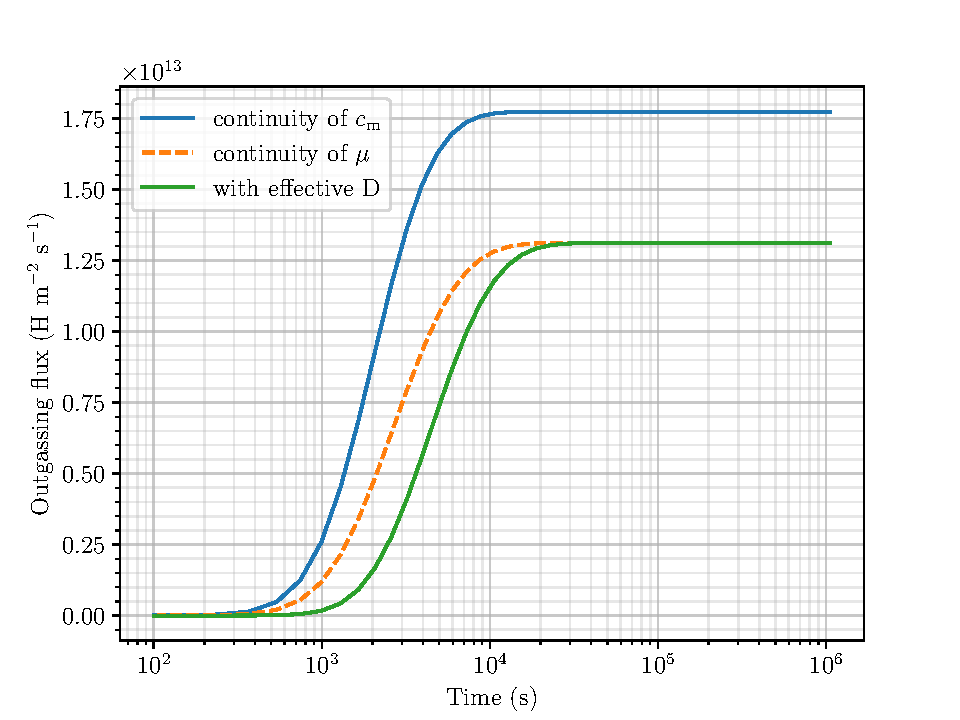
\includegraphics[width=0.5\linewidth]{Figures/Chapter3/monoblocks/interface_condition/cu_eurofer/comparison_fluxes_cu_eurofer.pdf}
     }
    \caption{Influence of chemical potential conservation}
    \label{fig: influence of mu bi material}
\end{figure*}

In this case, the conservation of chemical potential resulted in higher steady-state concentration gradients (see Figure \ref{fig: solute profiles w cu}) due to the higher solubility of Cu.
For a given temperature (and therefore given diffusion coefficients), this implied an increase of the outgassing flux (see Figure \ref{fig: outgassing flux w cu}) compared to the case with concentration continuity.

\subsection{Cu/EUROFER case}

A \SI{4}{mm}-thick slab made of \SI{2}{mm} of Cu (referred as $\Omega_1$) and \SI{2}{mm} of EUROFER (referred as $\Omega_2$) at $T=\SI{600}{K}$ was simulated.
Contrarily to the previous case, since the solubility of EUROFER is lower than that of Cu, the steady-state concentration gradients (see Figure \ref{fig: solute profiles cu eurofer}) were lower compared to the case with concentration continuity.
The outgassing flux was therefore lower in the case of chemical potential conservation (see Figure \ref{fig: outgassing flux cu eurofer}).



\subsection{Identification technique}
Assuming the diffusion coefficients are known, the solubility coefficients in both materials can be identified by determining an effective diffusion coefficient.

The steady-state flux $\varphi_\infty$ can be expressed from Equations \ref{eq:MES c} and \ref{eq: MES c coefficients} as follow:
\begin{subequations}
    \begin{align}
        \varphi_\infty &= -D_2 \nabla c_2 =  -D_1 \nabla c_1 \\
        &= -D_2 a_2 \frac{c_\mathrm{m}(x=0)}{L} = -D_1 a_1 \frac{c_\mathrm{m}(x=0)}{L}\\
        &= -a_0 D_\mathrm{eq} \frac{c_\mathrm{m}(x=0)}{L}
    \end{align}
    \label{eq: steady state flux 1}
\end{subequations}

If this method allows to measure solubilities, it is however not always convenient considering the time required to reach steady-state.
One way to overcome this difficulty is to compute an equivalent effective diffusion coefficient noted $D_\mathrm{eff}$.
$D_\mathrm{eff}$ is computed by assuming an homogeneous material and a linear steady state profile.
The steady-state flux can therefore be written as:
\begin{subequations}
    \begin{align}
        \varphi_\infty &= -D_\mathrm{eff} \nabla c \\
        &= -D_\mathrm{eff} \frac{c_\mathrm{m}(x=L) - c_\mathrm{m}(x=0)}{L} \\
    \end{align}
    \label{eq: steady state flux 2}
\end{subequations}

By combining Equations \ref{eq: steady state flux 1} and \ref{eq: steady state flux 2}, $D_\mathrm{eff}$ reads:
\begin{equation}
    D_\mathrm{eff} = \frac{a_0 \; D_\mathrm{eq} \; c_\mathrm{m}(x=0) }{c_\mathrm{m}(x=L) - c_\mathrm{m}(x=0)}
\end{equation}

By fitting measurements of the outgassing flux with either an analytical transient solution or a simulation code (see Figures \ref{fig: outgassing flux w cu} and \ref{fig: outgassing flux cu eurofer}), one can estimate $D_\mathrm{eff}$ and therefore the coefficient $a_0$ which can finally be correlated to material properties (see Equation \ref{eq: MES c coefficients}).

However, some discrepancies were found between this method and the actual outgassing curve during the transient phase.
One way of getting rid of these is to fit the curve with an analytical solution of transient mass transfer in a 1D composite slab with conservation of chemical potential.
This can be utterly complex and is well beyond the scope of this study.

Moreover, surface effects and the presence of traps often complicate the analysis of the experimental data.
Therefore, a more thorough identification technique would be to use embedded hydrogen transport codes such as FESTIM in a parametric optimisation algorithm as described in previous work \sidecite{delaporte-mathurin_parametric_nodate}.
Such a process could be able to determine materials properties such as diffusion coefficients, solubilities and trap densities.

This implementation of chemical potential continuity was applied to a test case in order to simulate hydrogen transport an ITER-like monoblock.
For this application, trapping of hydrogen in defects was taken into account.
The governing equations for hydrogen transport therefore read:

\begin{subequations}
    \begin{align}
        \frac{\partial c_\mathrm{m}}{\partial t} &=\nabla \cdot\left(D(T) \nabla c_\mathrm{m}\right) + \varphi_\mathrm{imp} \cdot U(\textbf{x}) -\sum \frac{\partial c_{\mathrm{t}, i}}{\partial t} \\
        \frac{\partial c_{\mathrm{t}, i}}{\partial t} &=k(T) \cdot c_\mathrm{m} \cdot\left(n_{i}-c_{\mathrm{t}, i}\right)-p(T) \cdot c_{\mathrm{t}, i}
    \end{align}
\end{subequations}

where ${D(T)=D_0 \cdot \exp\big(-E_\mathrm{diff}/ (k_B \cdot T )\big)}$ is the diffusion coefficient in \si{m^2.s^{-1}}, $T$ the temperature in $\si{K}$ and ${k_B = \SI{8.617e-5}{eV.K^{-1}}}$ the Boltzmann constant, $c_{\mathrm{t}, i}$ is the concentration in \si{m^{-3}} of particles trapped in the i-th trap,
\begin{equation}
    k(T)=k_0\exp{\big(-E_{k} / (k_B \cdot T ) \big)}
\end{equation} and 
\begin{equation}
    p(T)=p_0\exp{\big(-E_{p}/ (k_B \cdot T )\big)}
\end{equation} 
are the trapping and detrapping rates expressed in \si{m^3.s^{-1}} and \si{s^{-1}} respectively, $n_i$ is the trap density in \si{m^{-3}}, $\varphi_\mathrm{imp}$ is the implanted particle flux in \si{m^{-2}.s^{-1}} and $U(\textbf{x})$ is the spatial distribution of the implanted particle flux.

The thorough description of this model as well as the verification of its implementation in FESTIM is given in \sidecite{delaporte-mathurin_finite_2019}.

The source term $\varphi_\mathrm{imp}$ is equal to \SI{5e23}{m^{-2}.s^{-1}} and its spatial distribution is:

\begin{equation}
    U(\textbf{x}) = \begin{cases}
    R_p^{-1},& \text{ if } x < R_p\\
    0,& \text{ else }
    \end{cases}
\end{equation}
where $R_p = \SI{2.5}{nm}$ is the implantation range.
Since the implantation range is very small compared to the monoblock dimensions, this source is equivalent to applying a Dirichlet boundary condition on the exposed surface \sidecite{delaporte-mathurin_parametric_2020}.
The value of this boundary condition therefore depends on $\varphi_\mathrm{imp}$, the implantation range $R_p$ and the diffusion coefficient $D$.


The chemical potential is conserved across interfaces by ensuring Equations \ref{eq: flux conservation} and \ref{eq: c/s conservation} where 
\begin{equation}
    {S = S_0 \cdot \exp\big(-E_S/ (k_B \cdot T )\big)}
\end{equation} is the solubility coefficient in \si{m^{-3}.Pa^{-0.5}}.

A comparison test was first performed and the FESTIM code was compared to TMAP7 \sidecite{longhurst_tmap7_2008} and Abaqus on a 1D case.
2D simulations of ITER-like monoblocks were then performed.
The influence of interface conditions on hydrogen inventory was studied in both cases.

The materials properties that have been set are detailed in Table \ref{tab:materials properties_1} and their thermal dependency is shown on Figure \ref{fig:properties_1}.
The trap properties in each material are detailed in Table \ref{tab:traps monoblock_1}.
All traps are homogeneously distributed in the materials, except for Trap 2 which is only located in the first micrometre behind the plasma facing surface $\Gamma_\mathrm{top}$ (see Figure \ref{fig: monoblock geometry}) to account for damage creation.


\begin{figure*}
     \subfloat[1D geometry \label{fig: monoblock 1D geometry}]{%
        \begin{overpic}[width=0.5\linewidth]{Figures/Chapter3/monoblocks/interface_condition/iter case/Monoblock 1D.pdf}
            \put(40, 50){\SI{6}{mm}}
            \put(40, 8){W}
            \put(62, 50){\SI{1}{mm}}
            \put(65, 8){Cu}
            \put(72, 50){\SI{1.5}{mm}}
            \put(72, 8){CuCrZr}
            \put(6, 25){\large$\Gamma_\mathrm{top}$}
            \put(85, 25){\large$\Gamma_\mathrm{coolant}$}
        \end{overpic}
     }
     \subfloat[2D geometry  \label{fig: monoblock 2d geometry}]{%
        \begin{overpic}[width=0.5\linewidth]{Figures/Chapter3/monoblocks/interface_condition/iter case/monoblock_sketch.pdf}
            \put(42, 5){\SI{28}{mm}}
            \put(97, 50){\SI{28}{mm}}
            \put(10, 32){\SI{13.5}{mm}}
            \put(42, 62){ \diameter \SI{12}{mm}}
            \put(42, 71){ \diameter \SI{15}{mm}}
            \put(42, 76){ \diameter \SI{17}{mm}}
            \put(20, 80){\large$\Gamma_\mathrm{top}$}
            \put(4, 60){\large$\Gamma_\mathrm{lateral}$}
            \put(78, 60){\large$\Gamma_\mathrm{lateral}$}
            \put(40, 41){\large$\Gamma_\mathrm{coolant}$}
        \end{overpic}
     }
     \caption{Monoblock geometry showing W armour \cruleme[grey]{0.3cm}{0.3cm}, Cu interlayer \cruleme[orange]{0.3cm}{0.3cm}, CuCrZr alloy cooling pipe  \cruleme[yellow]{0.3cm}{0.3cm}}\label{fig: monoblock geometry}
\end{figure*}

\begin{table*}
    \centering
    \begin{tabular}{p{1.7cm}  R{3cm}  R{3cm}  R{1.8cm}  R{1cm} R{1.8cm}  R{1cm}}
         & \multicolumn{2}{c}{Thermal properties} & \multicolumn{4}{c}{Hydrogen transport properties}\\
        \hline
        Material & $\rho \cdot C_p \newline(\si{J.K^{-1}.m^{-3}})$ & $\lambda \newline(\si{W.m^{-1}.K^{-1}})$ & $D_0 \newline(\si{m^2.s^{-1}})$ & $E_\mathrm{diff} \newline(\si{eV})$ & $S_0 \newline(\si{m^{-3}.Pa^{-0.5}})$ & $E_\mathrm{S} \newline(\si{eV})$\\
        \hline
        \\
        W \cite{frauenfelder_solution_1969}& %
        $5.1\times 10^{-6} \cdot T^3 \newline - 8.3\times 10^{-2}\cdot T^2 \newline + 6.0 \times 10^{2}\cdot T \newline +2.4\times 10^6$ &%
        $-7.8\times 10^{-9}\cdot T^3 \newline %
        +5.0\times 10^{-5}\cdot T^2 \newline%
        -1.1\times 10^{-1} \cdot T \newline%
        +1.8\times 10^{2}$ &%
        $2.4\times 10^{-7}$ & 0.39 &%
        $1.87\times 10^{24}$ & 1.04\\
        \\
        Cu \cite{reiter_compilation_1996}&%
        $1.7\times 10^{-4}\cdot T^3\newline %
        +6.1\times 10^{-2}\cdot T^2\newline %
        +4.7\times 10^2\cdot T\newline %
        +3.5\times 10^6$ &%

        $-3.9\times 10^{-8}\cdot T^3\newline %
        +3.8\times 10^{-5}\cdot T^2\newline %
        -7.9\times 10^{-2}\cdot T\newline %
        +4.0\times 10^2 $&%

        $6.6\times 10^{-7}$ &%
        0.39&%
        $3.14\times 10^{24}$ & 0.57\\
        \\
        CuCrZr \cite{serra_hydrogen_1998}& %
        $-1.8\times 10^{-4}\cdot T^3 \newline %
        +1.5\times 10^{-1}\cdot T^2\newline %
        +6.2\times 10^2\cdot T\newline %
        +3.5\times 10^6$ &%

        $5.3\times 10^{-7}\cdot T^3\newline %
        -6.5\times 10^{-4}\cdot T^2\newline %
        +2.6\times 10^{-1}\cdot T\newline %
        +3.1\times 10^2$ & %

        $3.9\times 10^{-7}$ & %
        0.42&%
        $4.28\times 10^{23}$ & 0.39\\
        \\
        EUROFER \cite{aiello_hydrogen_2002} & %
        - & - &
        $1.5\times 10^{-7}$ & %
        0.15 & %
        $6.14\times 10^{20}$ & 0.25
        \\
        \\
    \end{tabular}
    \caption{Materials properties used in the simulations. Thermal properties are fitted from ANSYS.}
    \label{tab:materials properties_1}
\end{table*}

\begin{figure}
    \centering
    \begin{subfigure}{0.75\linewidth}
        \centering
        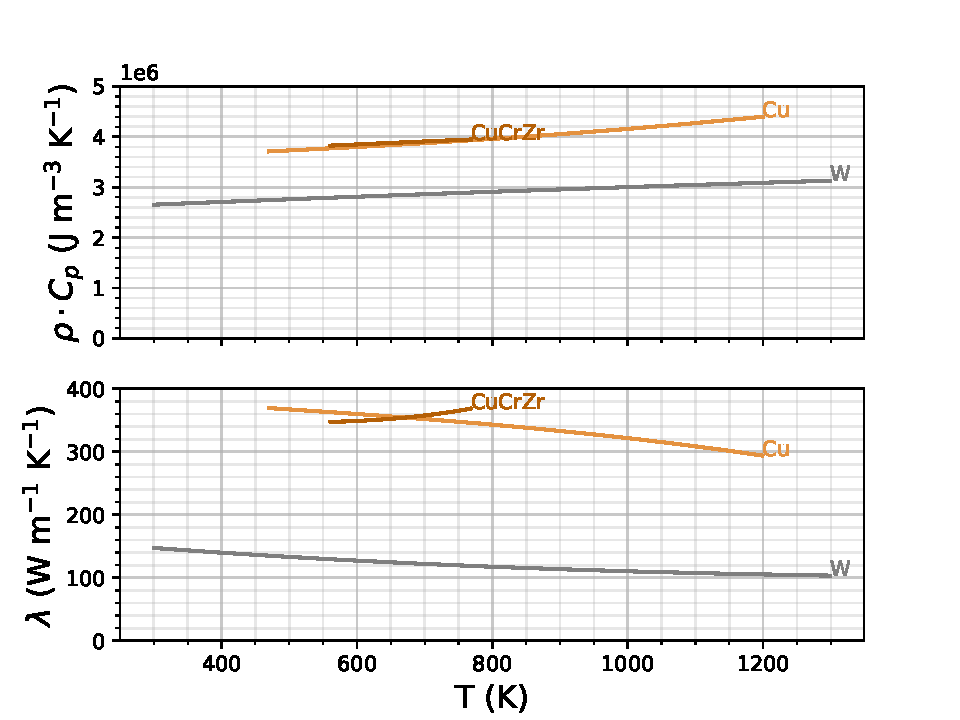
\includegraphics[width=\linewidth]{Figures/Chapter3/monoblocks/interface_condition/iter case/thermal_prop.pdf}
        \caption{Thermal properties}
    \end{subfigure}
    \begin{subfigure}{0.75\linewidth}
        \centering
        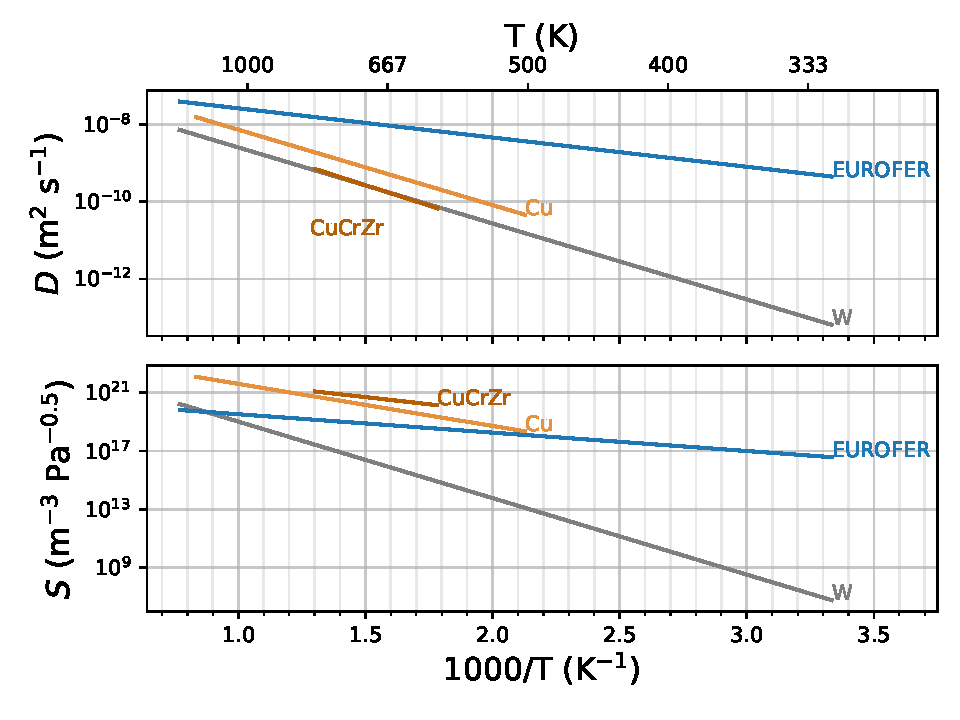
\includegraphics[width=\linewidth]{Figures/Chapter3/monoblocks/interface_condition/H_properties.pdf}
        \caption{H transport properties}
    \end{subfigure}
    \caption{Material properties used in the simulations \cite{frauenfelder_solution_1969, reiter_compilation_1996, serra_hydrogen_1998, aiello_hydrogen_2002}}
    \label{fig:properties_1}
\end{figure}

\begin{table*}
    \centering
    \begin{tabular}{L{1.5cm} L{1.5cm} R{1.6cm} R{1.1cm} R{1.6cm} R{1.1cm} R{2cm}}
         & Material & $k_0 (\si{m^3.s^{-1}})$ &  $E_k (\si{eV})$ & $p_0 (\si{s^{-1}})$ & $E_p (\si{eV})$ & $n_i (\si{at.fr.})$ \\
        \hline
        \\
        Trap 1 & W & $3.8 \times 10^{-17}$ & 0.39 & $8.4 \times 10^{12}$& 1.20 & $5.0 \times 10^{-4}$ \\
        \\
       Trap 2 & W & $3.8 \times 10^{-17}$ & 0.39 & $8.4 \times 10^{12}$& 1.40 & $5.0 \times 10^{-3}$ \\
        \\
        Trap 3 & Cu & $6.0 \times 10^{-17}$ & 0.39 & $8.0 \times 10^{13}$ & 0.50 &$5.0 \times 10^{-5}$\\
        \\
        Trap 4 & CuCrZr & $1.2\times 10^{-16}$ & 0.42 & $8.0 \times 10^{13}$ & 0.50 &$5.0 \times 10^{-5}$\\
        \\
        Trap 5 & CuCrZr & $1.2\times 10^{-16}$ & 0.42 & $8.0 \times 10^{13}$ & 0.83 &$4.0 \times 10^{-2}$\\
        \\
    \end{tabular}
    \caption{Traps properties used in the simulations \cite{hodille_macroscopic_2015, dolan_assessment_1994}}
    \label{tab:traps monoblock_1}
\end{table*}


\subsection{1D case and comparison with TMAP7 and Abaqus}

\begin{figure}
    \centering
    \begin{subfigure}{0.5\linewidth}                              
        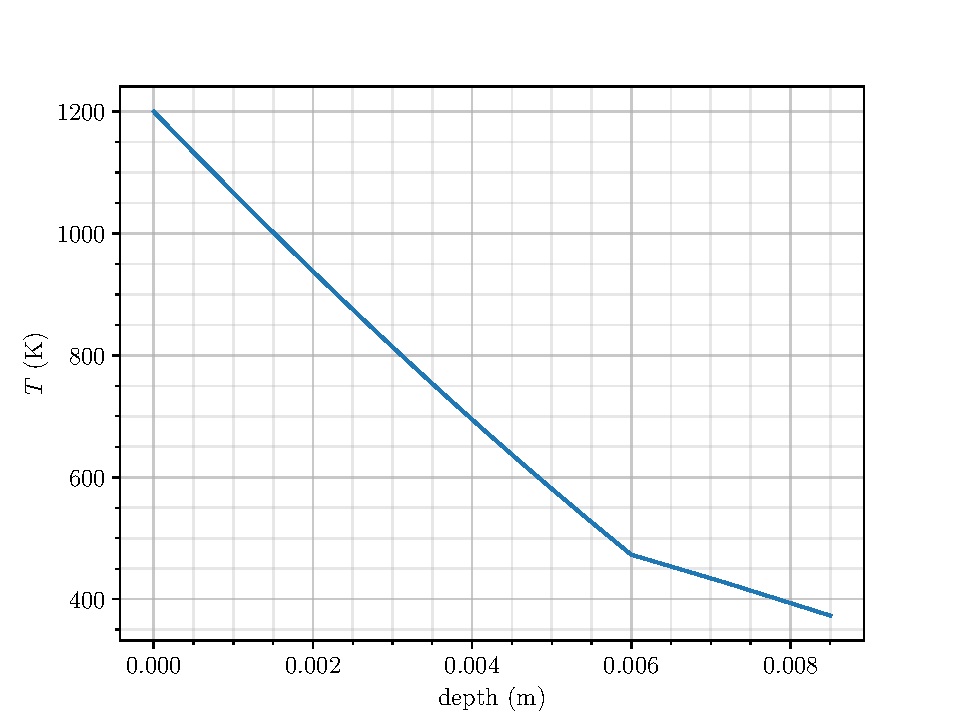
\includegraphics[width=\linewidth]{Figures/Chapter3/monoblocks/interface_condition/iter case/temperature_1D.pdf}
        \caption{1D case}
        \label{fig: 1D temperature}
    \end{subfigure}%
    \begin{subfigure}{0.5\linewidth}                          
        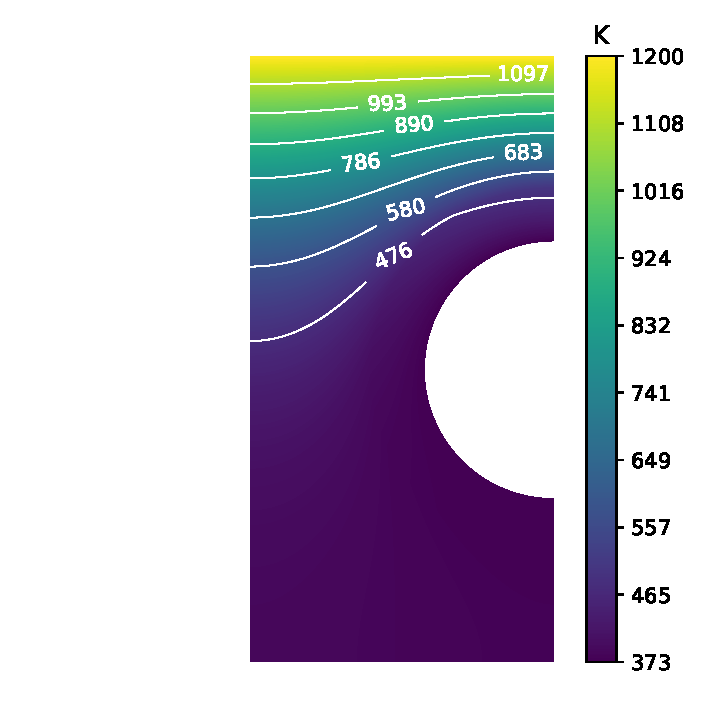
\includegraphics[width=\linewidth]{Figures/Chapter3/monoblocks/interface_condition/iter case/temperature_field_2d.pdf}
        \caption{2D case}
        \label{fig: 2D temperature}
    \end{subfigure}%
    \caption{Monoblock temperature simulated by FESTIM}
    \label{fig: temperature}
\end{figure}

\begin{figure}
    \centering
    \begin{subfigure}{1\linewidth}
        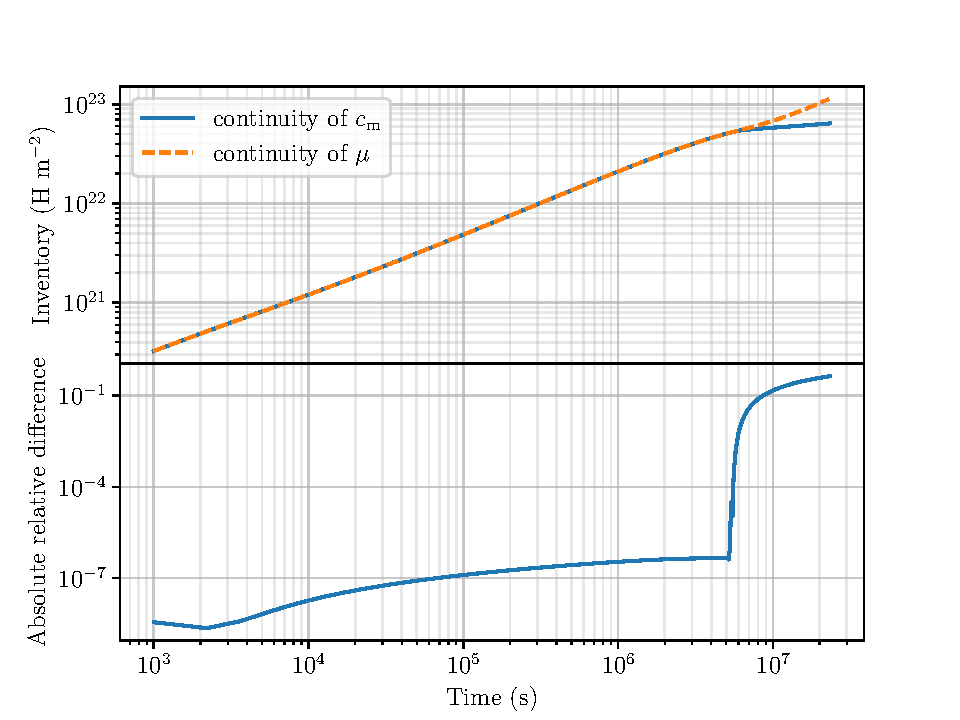
\includegraphics[width=\linewidth]{Figures/Chapter3/monoblocks/interface_condition/iter case/comparison_inventory_1d.pdf}
        \caption{1D case}
        \label{fig: 1D inventories}
    \end{subfigure}
    \begin{subfigure}{1\linewidth} 
        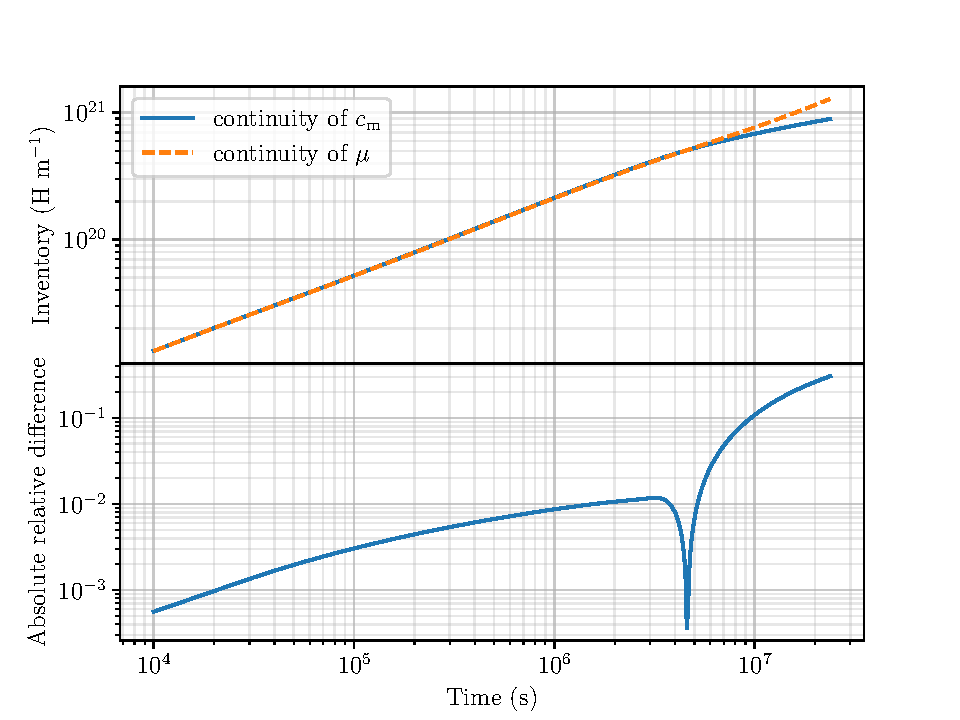
\includegraphics[width=\linewidth]{Figures/Chapter3/monoblocks/interface_condition/iter case/comparison_inventory_2d.pdf}
        \caption{2D case}
        \label{fig: 2D inventories}
    \end{subfigure}
    \caption{Influence of chemical potential conservation on hydrogen inventory}
\end{figure}

\begin{figure}
    \centering
    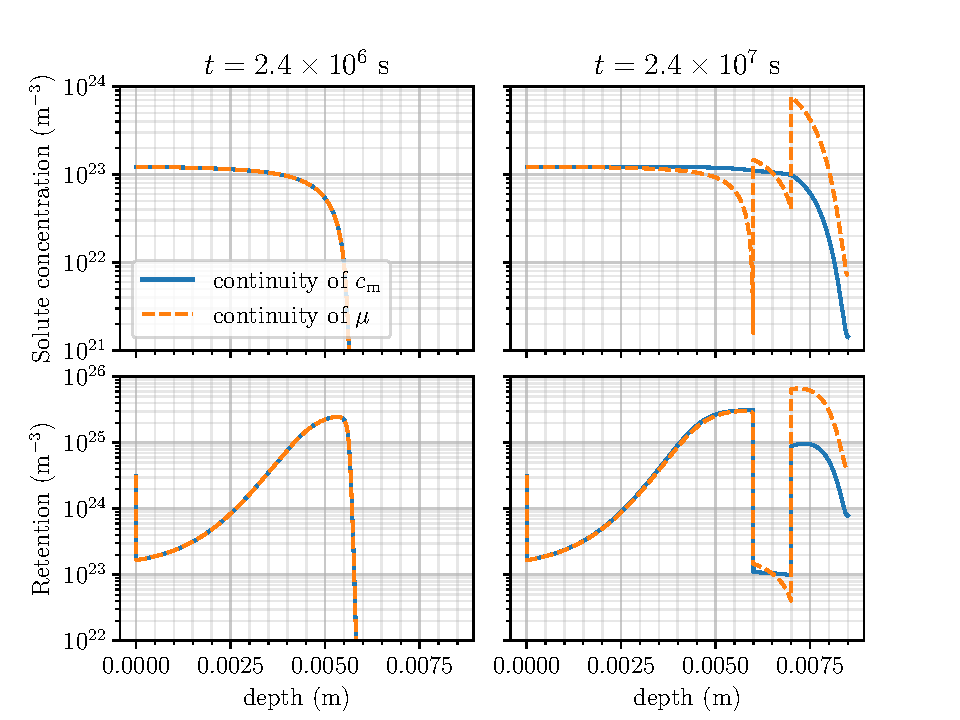
\includegraphics[width=\linewidth]{Figures/Chapter3/monoblocks/interface_condition/iter case/comparison_profiles.pdf}
    \caption{Comparison of concentrations profiles at several times}
    \label{fig: concentrations profiles 1D}
\end{figure}

\begin{figure}
    \centering
    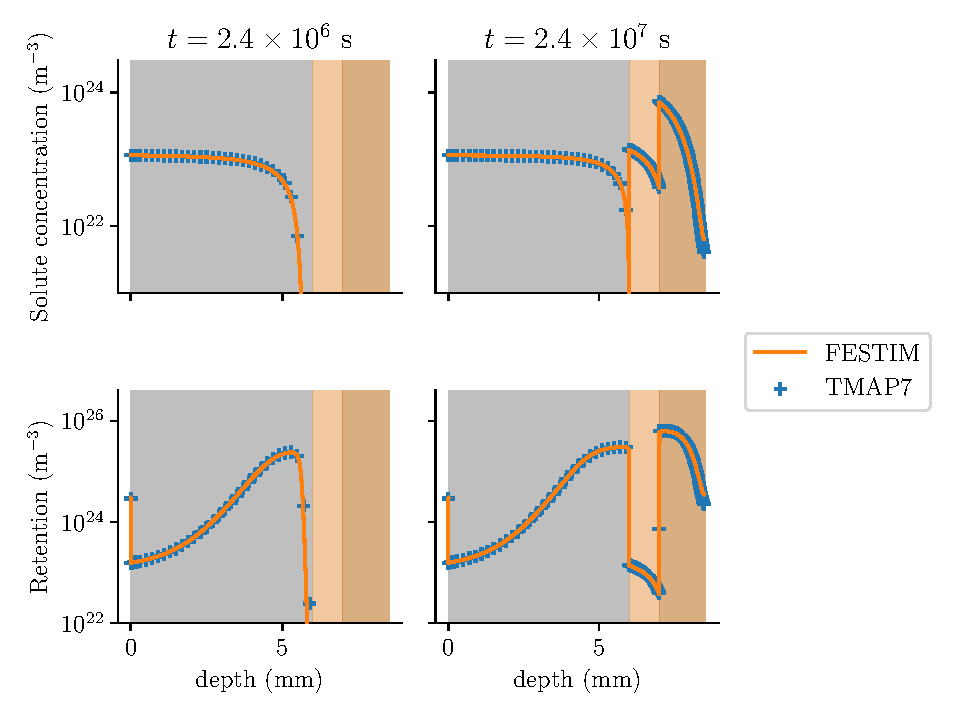
\includegraphics[width=\linewidth]{Figures/Chapter3/monoblocks/interface_condition/iter case/comparison_codes.pdf}
    \caption{Comparison of results provided by FESTIM, TMAP7 and ABAQUS}
    \label{fig: code comparison}
\end{figure}

The 1D simulation case is a \SI{8.5}{mm}-thick composite slab made of W, Cu and CuCrZr (see Figure \ref{fig: monoblock 1D geometry}).
The plasma facing surface $\Gamma_\mathrm{top}$ is located at $x=\SI{0}{mm}$ and the surface cooled by water $\Gamma_\mathrm{coolant}$ is located at $x=\SI{8.5}{mm}$.


The boundary conditions are detailed in Equation \ref{eq: 1D BCs}.

\begin{subequations}
    \begin{align}
    T &= \SI{1200}{K}\quad \text { on } \Gamma_\mathrm{top}\\
    c_\mathrm{m} &=  \frac{\varphi_\mathrm{imp} \cdot R_p}{D} \quad \text { on } \Gamma_\mathrm{top}\\
    T &= \SI{373}{K} \quad \text { on } \Gamma_\mathrm{coolant}\\
    -D \nabla c_\mathrm{m} \cdot \vec{n} &= K_\mathrm{CuCrZr} \cdot c_\mathrm{m}^{2} \quad \text { on } \Gamma_\mathrm{coolant}  
    \end{align}
    \label{eq: 1D BCs}
\end{subequations}
with $\varphi_\mathrm{imp} = \SI{5e23}{m^{-2}.s^{-1}}$ the implanted particle flux, $R_p = \SI{1.25}{nm}$ the implantation depth, $\vec{n}$ the normal vector and $K_\mathrm{CuCrZr} = 2.9 \times 10^{-14}\cdot \exp{(-1.92/(k_B\cdot T))}$ the recombination coefficient of the CuCrZr (in vacuum) expressed in \si{m^4.s^{-1}} \sidecite{anderl_deuterium_1999}.

The Dirichlet boundary condition on $\Gamma_\mathrm{top}$ for the hydrogen transport corresponds to a flux balance between the implanted flux and the flux that is retro-desorbed at the surface.
The details can be found in \sidecite{delaporte-mathurin_parametric_2020}.

A comparison test was made with the codes TMAP7 and Abaqus with this set of parameters and very good agreement was found between the two codes (see Figure \ref{fig: code comparison}).



Two simulations were run, one ensuring mobile concentration $c_\mathrm{m}$ continuity at interfaces and the other ensuring the continuity of chemical potential $\mu$.

Up to \SI{5e6}{s}, the total hydrogen inventory was found to be insensitive to the conservation of chemical potential (see Figure \ref{fig: 1D inventories}).
It is only after this implantation that the inventory of the simulation with continuity of chemical potential started to diverge.
At $t=\SI{2.4e7}{s}$, the inventory with continuity of $\mu$ was more than two times higher than that of the one with continuity of $c_\mathrm{m}$.
This is explained by the high solubility ratio between Cu and CuCrZr leading to a higher concentration of mobile particles in CuCrZr and therefore a higher trapping rate.
Before reaching the W/Cu interface, the $c_\mathrm{m}$ and retention profiles are identical regardless of the interface condition (see Figure \ref{fig: concentrations profiles 1D}).
Once this interface is reached, the $c_\mathrm{m}$ profiles are affected by the interface condition.
However, even then, the trap density in Cu being low compared to other materials, the global inventory is not affected much.
For these two reasons, the inventories are identical before \SI{5e6}{s}.

\subsection{2D case}
The boundary conditions for the 2D case are similar with an additional Dirichlet boundary condition on $\Gamma_\mathrm{lateral}$.
This boundary condition accounts for recombination on the lateral sides of the monoblock.
\begin{subequations}
    \begin{align}
        T &=  \SI{1200}{K}\quad \text { on } \Gamma_\mathrm{top}\\
        c_\mathrm{m} &=  \frac{\varphi_\mathrm{imp} \cdot R_p}{D}\quad \text { on } \Gamma_\mathrm{top}\\
        T &= \SI{373}{K}\quad \text { on } \Gamma_\mathrm{coolant}\\
        -D \nabla c_\mathrm{m} \cdot \vec{n} &= K_\mathrm{CuCrZr} \cdot c_\mathrm{m}^{2} \quad \text { on } \Gamma_\mathrm{coolant} \\
        c_\mathrm{m} &= 0 \quad \text { on } \Gamma_\mathrm{lateral}
    \end{align}
\end{subequations}

with $\varphi_\mathrm{imp} = \SI{5e23}{m^{-2}.s^{-1}}$ the implanted particle flux, $R_p = \SI{1.25}{nm}$ the implantation depth, $\vec{n}$ the normal vector and $K_\mathrm{CuCrZr} = 2.9 \times 10^{-14}\cdot \exp{(-1.92/(k_B\cdot T))}$ the recombination coefficient of the copper alloy (in vacuum) expressed in \si{m^4.s^{-1}} \sidecite{anderl_deuterium_1999}.


\begin{figure}s
    \centering
    \begin{subfigure}{0.5\linewidth}
        \centering
        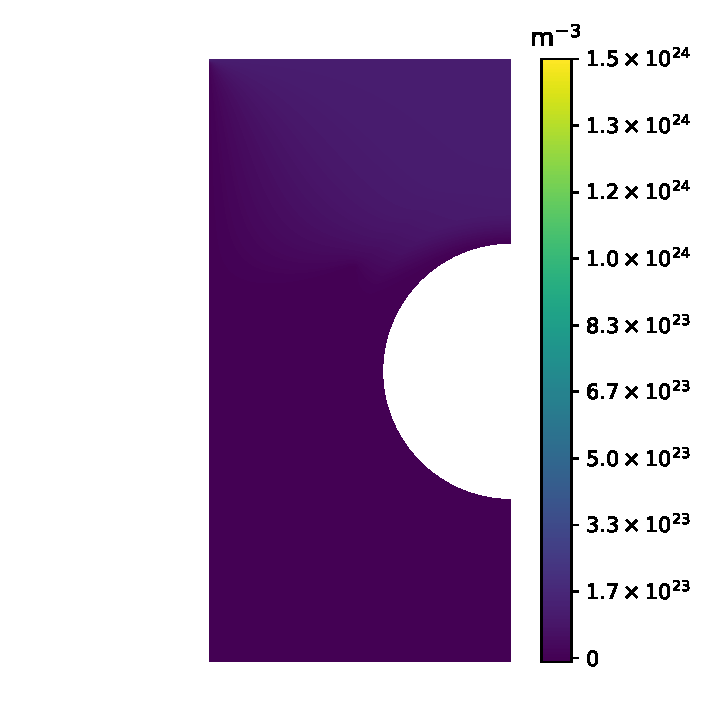
\includegraphics[width=\linewidth]{Figures/Chapter3/monoblocks/interface_condition/iter case/solute_c.pdf}
        \caption{$c_\mathrm{m}$ (continuity of $c_\mathrm{m}$)}
    \end{subfigure}%
    \begin{subfigure}{0.5\linewidth}
        \centering
        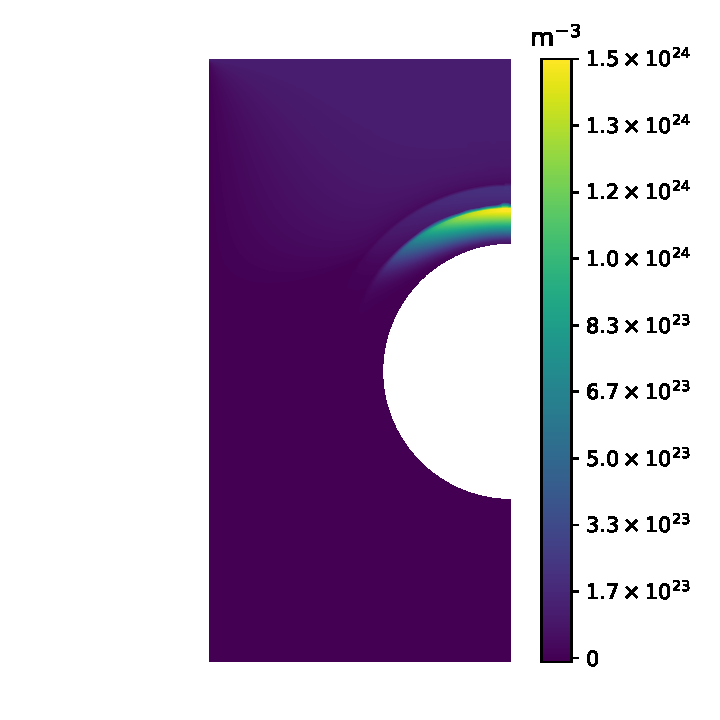
\includegraphics[width=\linewidth]{Figures/Chapter3/monoblocks/interface_condition/iter case/solute_mu.pdf}
        \caption{$c_\mathrm{m}$ (continuity of $\mu$)}
    \end{subfigure}
    \begin{subfigure}{0.5\linewidth}
        \centering
        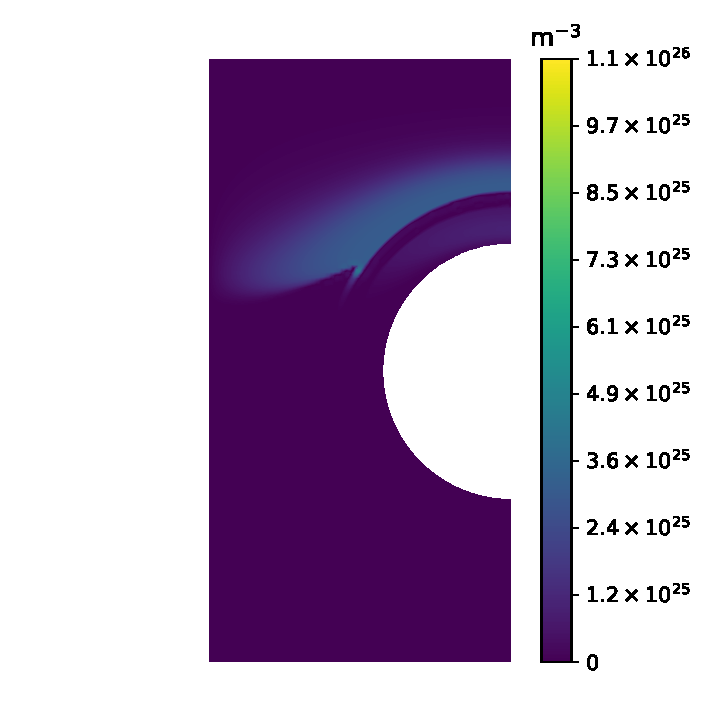
\includegraphics[width=\linewidth]{Figures/Chapter3/monoblocks/interface_condition/iter case/retention_c.pdf}
        \caption{Retention (continuity of $c_\mathrm{m}$)}
    \end{subfigure}%
    \begin{subfigure}{0.5\linewidth}
        \centering
        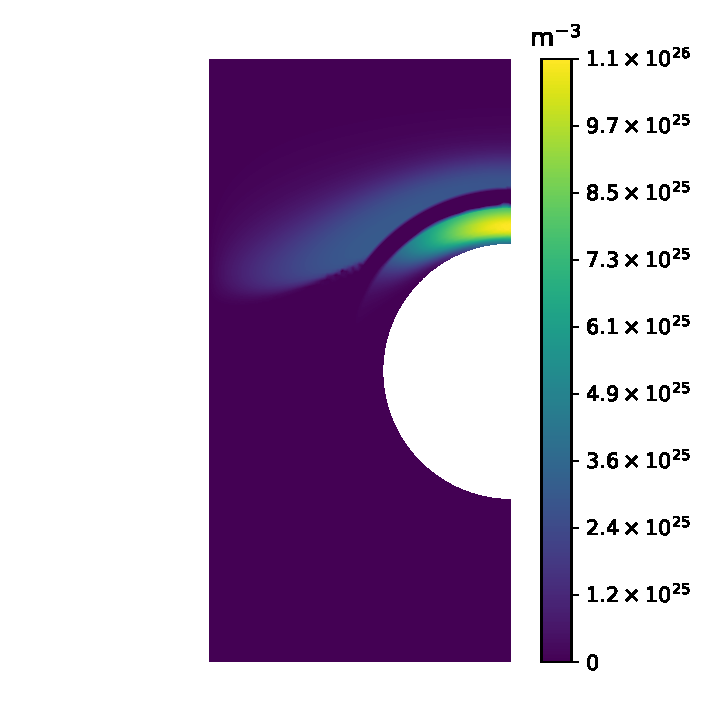
\includegraphics[width=\linewidth]{Figures/Chapter3/monoblocks/interface_condition/iter case/retention_mu.pdf}
        \caption{Retention (continuity of $\mu$)}
    \end{subfigure}
    \caption{2D concentration fields at $t=\SI{2.4e7}{s}$}
    \label{fig: concentrations fields 2d}
\end{figure}

The concentrations fields (see Figure \ref{fig: concentrations fields 2d}) showed results similar to those obtained in the 1D case (see Figure \ref{fig: concentrations profiles 1D}).
The interface condition had no influence whatsoever on the mobile particle concentration $c_\mathrm{m}$ in the W.
However, $c_\mathrm{m}$ was higher in Cu and CuCrZr in the case with chemical potential conservation (up to \SI{1.5e24}{m^{-3}} in CuCrZr at $t=\SI{2.4e7}{s}$).
As in the 1D case, this increase of $c_\mathrm{m}$ lead to an increase of the trap occupancy and therefore an increase of the local retention.

The hydrogen inventories in the monoblock were found to be identical for most of the implantation time (see Figure \ref{fig: 2D inventories}).
It was only after \SI{5e6}{s} that the inventory with chemical potential conservation was significantly higher than the one with $c_\mathrm{m}$ continuity at interfaces.

In both the 1D and 2D case, the flux which is retro-desorbed from the monoblock to the plasma does not depend on the interface conditions since interface are far from the exposed surface.
Moreover, outgassing flux through the cooling pipe greatly depends on the boundary condition imposed at the cooling surface.
Therefore, in order to assess the impact of interface conditions on the outgassing flux through the cooling pipe, uncertainties must first be lift regarding the recombination process occurring on surfaces in contact with water.

\subsection{Summary}
